\documentclass[oneside]{book}
\usepackage{epsfig,graphicx} % Required for inserting images
\usepackage{amsmath}
\usepackage{amsthm}
\usepackage{amssymb}
\usepackage{subcaption}
\usepackage[spanish,mexico]{babel}
\usepackage[bookmarksopen]{hyperref}
\usepackage[utf8]{inputenc}
\usepackage{array}
\usepackage{listings} %Soporte para código
\usepackage[left=2cm,right=2cm,top=1.8cm,bottom=2.3cm]{geometry}
\usepackage{titlesec}
\usepackage{fancyhdr} 
\usepackage{enumitem}
\usepackage{multicol}
\usepackage{multirow}           % Permits header customization. See header section below.
\usepackage{wrapfig}
\usepackage{circuitikz}
\usepackage{xcolor}

% ---definición de los paquetes--
\fancypagestyle{plain}{
    \lhead{}
    \fancyhead[R]{\thepage}
    \fancyhead[L]{}
    \renewcommand{\headrulewidth}{0pt}
    \fancyfoot{}
}
\pagestyle{fancy}
\fancyhead[R]{	\thepage}
\fancyhead[L]{}
% Definir el tamaño del título del capítulo
\titleformat{\chapter}[display]
  {\normalfont\huge\bfseries} % Estilo del título
  {\chaptertitlename\ \thechapter}{1pt}{\Large} % Tamaño del título
  \titlespacing*{\chapter}{0pt}{-20pt}{20pt} % Ajustar el espaciado

\title{Tarea 03: Circuitos y logica de primer orden.}
\author{Ramírez Mendoza Joaquín Rodrigo\\
Villalobos Juárez Gontran Eliut\\
Treviño Puebla Héctor Jerome}
\date{\today}
% ---Inicio de la portada
\begin{document}
\begin{titlepage}
	\begin{minipage}{3cm}
		\begin{center}
			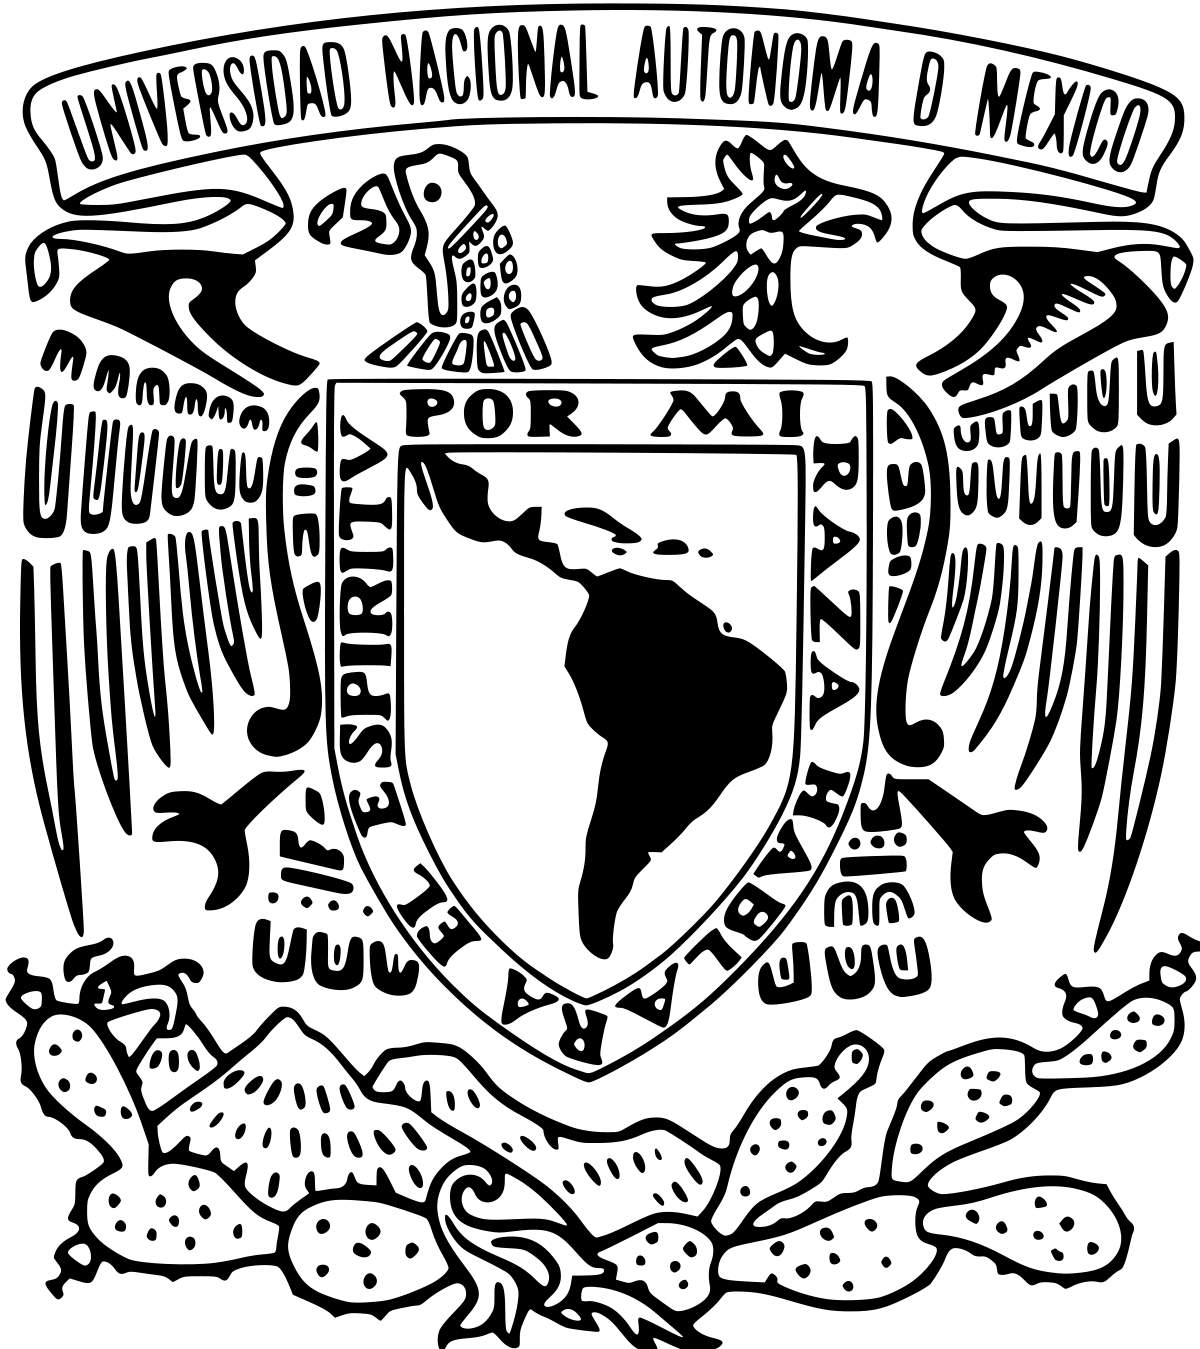
\includegraphics[height = 0.14\textheight]{recursos/Logo_UNAM.png}\par
		\end{center}
	\end{minipage}\hfill
	\begin{minipage}{10cm}

	\end{minipage}\hfill
	\begin{minipage}{3cm}
		\begin{center}
			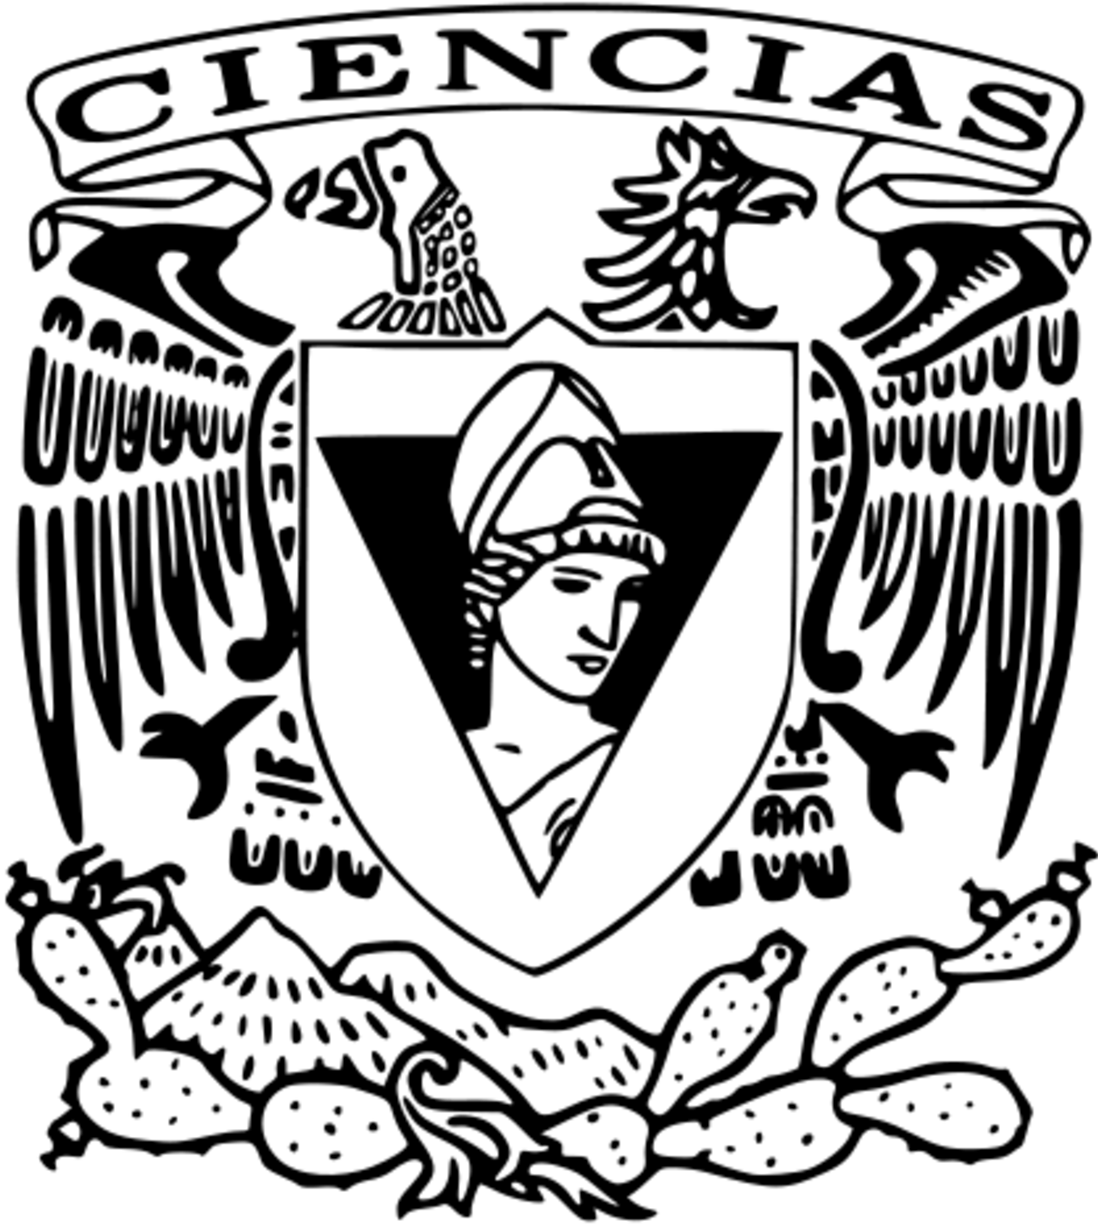
\includegraphics[height = 0.14\textheight]{recursos/Logo_FC.png}\par
		\end{center}
	\end{minipage}
	\centering
	\vspace{1cm}

	{\bfseries\LARGE Universidad Nacional Autónoma de México \par}

	\vspace{1cm}
	{\scshape\Large Facultad de Ciencias \par}
	\vspace{1cm}
	{\scshape\Large Estructuras Discretas \par}
	\vspace{1cm}
	{\scshape\Large Licenciatura en Ciencias de la Computación \par}
	\vspace{1cm}
	{\scshape\Huge Tarea 03: Circuitos y logica de primer orden.  \par}
	\vspace{3cm}
	{\itshape\Large Primer Parcial \par}
	\vfill
	{\Large Autores: \par}
	{\Large Ramírez Mendoza Joaquín Rodrigo \par}
	{\Large Villalobos Juárez Gontran Eliut\par}
	{\Large Treviño Puebla Héctor Jerome \par}
	\vfill
	{\Large Agosto 2024 \par}
\end{titlepage}
% ---Fin de la portada de la portada
\maketitle

% Introducir aquí sus capítulos
% ------∨∨∨∨∨∨∨∨∨∨∨∨∨∨∨--------
\chapter*{Asumiendo los axiomas de un álgebra booleana  A = \{{0,1},+,$\cdot$\} demostrar las siguientes propiedades:}
\begin{enumerate}[label=\alph*)]
	\item Idempotencia: $x+x = x $ y $ xx = x$.
	\item Idempotencia de complemento:  $(\bar{\bar{x}})= x$.
	\item Elemento dominante: $x+1 = 1$ y $x0 = 0$.
	\item Absorción: $x+xy = x$ y $x(x+y) = x$.
\end{enumerate}
\begin{multicols}{2}
	\noindent
	$\underline{Dem \;a)}:\; \text{Sea $x$ un elemento del álgebra booleana}$
	\begin{align*}
		(x+x) & =(x+x)\cdot 1           \\
		      & =(x+x)\cdot (x+\bar{x}) \\
		      & =x + x\bar{x}           \\
		      & =x + 0                  \\
		      & =x\; \blacksquare       \\
	\end{align*}

	\columnbreak

	\noindent
	$\underline{Dem}:\; \text{Sea $x$ un elemento del álgebra booleana}$
	\begin{align*}
		xx & =xx+0              \\
		   & =xx+(x\bar{x})     \\
		   & =x\cdot(x+\bar{x}) \\
		   & =x\cdot 1          \\
		   & =x                 \\
	\end{align*}
\end{multicols}
\begin{multicols}{2}
	\noindent
	$\underline{Dem \;b)}:\; \text{Sea $x$ un elemento del álgebra booleana}$
	\begin{align*}
		(\bar{\bar{x}}) & = x \\
	\end{align*}
\end{multicols}

\begin{multicols}{2}
	\noindent
	$\underline{Dem \;c)}:\; \text{Sea $x$ un elemento del álgebra booleana}$
	\begin{align*}
		(x+1) & = 1 \\
	\end{align*}

	\columnbreak

	\noindent
	$\underline{Dem}:\; \text{Sea $x$ un elemento del álgebra booleana}$
	\begin{align*}
		x0 & = 0 \\
	\end{align*}
\end{multicols}

\begin{multicols}{2}
	\noindent
	$\underline{Dem \;d)}:\; \text{Sea $x$ un elemento del álgebra booleana}$
	\begin{align*}
		(x+xy) & =x \\
	\end{align*}

	\columnbreak

	\noindent
	$\underline{Dem}:\; \text{Sea $x$ un elemento del álgebra booleana}$
	\begin{align*}
		x(x+y) & =x \\
	\end{align*}
\end{multicols}

\chapter*{Dibuja los circuitos lógicos para las siguientes expresiones}

Dibuja los circuitos lógicos para las siguientes expresiones:

\begin{enumerate}
    \item[(a)] $xyz \oplus x\overline{y}z$
    \item[(b)] $xy + x\overline{y}$
    \item[(c)] $xy\overline{z} + x\overline{yz}$
    \item[(d)] $\overline{x} + \overline{y} + xyz$
    
\end{enumerate}
 \begin{figure}[h!]
    \centering
    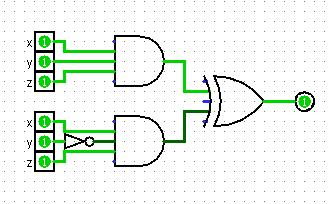
\includegraphics[width=\textwidth]{recursos/Ejercicio2/circuito_a.png}
    \caption{Circuito lógico para $xyz \oplus x\overline{y}z$}
\end{figure}
\newpage

\begin{figure}[h!]
    \centering
    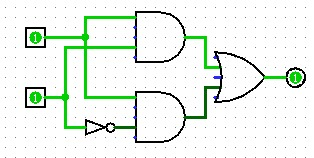
\includegraphics[width=\textwidth]{recursos/Ejercicio2/circuito_b.png}
    \caption{Circuito lógico para $xy + x\overline{y}$}
\end{figure}

\begin{figure}[h!]
    \centering
    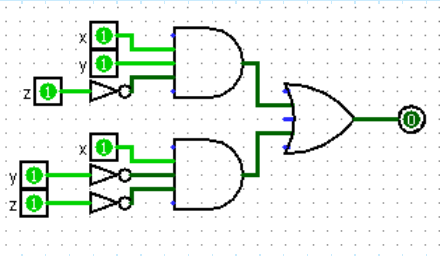
\includegraphics[width=\textwidth]{recursos/Ejercicio2/circuito_c.png}
    \caption{Circuito lógico para $xy\overline{z} + x\overline{yz}$}
\end{figure}

\begin{figure}[h!]
    \centering
    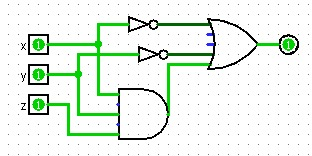
\includegraphics[width=\textwidth]{recursos/Ejercicio2/circuito_d.png}
    \caption{Circuito lógico para $\overline{x} + \overline{y} + xyz$}
\end{figure}




\chapter*{Utilizando mapas de Karnaugh, reducir las siguientes expresiones y dibujar los circuitos reducidos}

\section*{Problema}
Utilizando mapas de Karnaugh, reducir las siguientes expresiones y dibujar los circuitos reducidos:

\begin{enumerate}
    \item[(a)] $xy + x\overline{y}$
    \item[(b)] $\overline{x}y + \overline{xy}$
    \item[(c)] $xyz + \overline{x}yz$
    \item[(d)] $xy\overline{z} + x\overline{yz} + \overline{x}y\overline{z} + \overline{xyz}$
    \item[(e)] $\overline{xy} + \overline{x}y + xy$
    \item[(f)] $\overline{xy} + \overline{x}y + x + y$
\end{enumerate}

\section*{Soluciones}

\subsection*{(a) $xy + x\overline{y}$}

\begin{itemize}
    \item Mapa de Karnaugh:
\begin{center}
    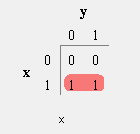
\includegraphics[width=0.3\textwidth]{recursos/Ejercicio3/mapas/mapa_a).png}
\end{center}

    \item Simplificación: \[ xy + x\overline{y} = x \]

    \item Circuito reducido:
\begin{center}
    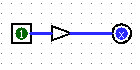
\includegraphics[width=0.4\textwidth]{recursos/Ejercicio3/circuito/circuito_a).png}
\end{center}
\end{itemize}

\subsection*{(b) $\overline{x}y + \overline{xy}$}

\begin{itemize}
    \item Mapa de Karnaugh:
\begin{center}
    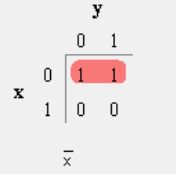
\includegraphics[width=0.4\textwidth]{recursos/Ejercicio3/mapas/mapa_b).png}
\end{center}

    \item Simplificación: \[ \overline{x}y + \overline{xy} = \overline{x} \]

    \item Circuito reducido:
\begin{center}
    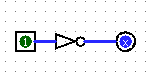
\includegraphics[width=0.3\textwidth]{recursos/Ejercicio3/circuito/circuito_b).png}
\end{center}
\end{itemize}

\subsection*{(c) $xyz + \overline{x}yz$}

\begin{itemize}
    \item Mapa de Karnaugh:
\begin{center}
    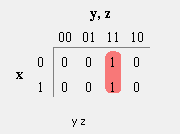
\includegraphics[width=0.4\textwidth]{recursos/Ejercicio3/mapas/mapa_c).png}
\end{center}

    \item Simplificación: \[ xyz + \overline{x}yz = yz \]

    \item Circuito reducido:
\begin{center}
    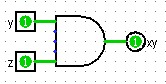
\includegraphics[width=0.3\textwidth]{recursos/Ejercicio3/circuito/circuito_c).png}
\end{center}
\end{itemize}

\subsection*{(d) $xy\overline{z} + x\overline{yz} + \overline{x}y\overline{z} + \overline{xyz}$}

\begin{itemize}
    \item Mapa de Karnaugh:
\begin{center}
    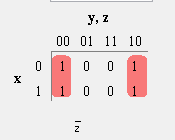
\includegraphics[width=0.4\textwidth]{recursos/Ejercicio3/mapas/mapa_d).png}
\end{center}

    \item Simplificación: \[ xy\overline{z} + x\overline{yz} + \overline{x}y\overline{z} + \overline{xyz} = \overline{z} \]

    \item Circuito reducido:
\begin{center}
    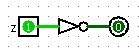
\includegraphics[width=0.3\textwidth]{recursos/Ejercicio3/circuito/circuito_d).png}
\end{center}
\end{itemize}

\subsection*{(e) $\overline{xy} + \overline{x}y + xy$}

\begin{itemize}
    \item Mapa de Karnaugh:
\begin{center}
    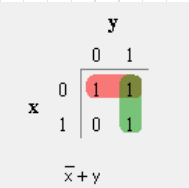
\includegraphics[width=0.3\textwidth]{recursos/Ejercicio3/mapas/mapa_e).png}
\end{center}

    \item Simplificación: \[ \overline{xy} + \overline{x}y + xy = \overline{x} + y \]

    \item Circuito reducido:
\begin{center}
    \includegraphics[width=0.3\textwidth]{recursos/Ejercicio3/circuito/ciurcuito_e).png}
\end{center}
\end{itemize}

\subsection*{(f) $\overline{xy} + \overline{x}y + x + y$}

\begin{itemize}
    \item Mapa de Karnaugh:
\begin{center}
    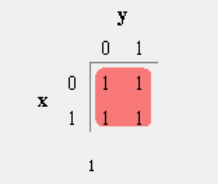
\includegraphics[width=0.3\textwidth]{recursos/Ejercicio3/mapas/mapa_f).png}
\end{center}

    \item Simplificación: \[ \overline{xy} + \overline{x}y + x + y = 1 \]

    \item Circuito reducido:
\begin{center}
    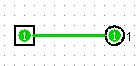
\includegraphics[width=0.3\textwidth]{recursos/Ejercicio3/circuito/circuito_f).png}

\end{center}
\end{itemize}



\chapter*{Ejercicio 4}

\textbf{4.}  Diseñar un circuito decodificador con 4 entradas para la siguiente tabla de verdad, donde - denota cualquier valor, 0 o 1:

\begin{center}
        \begin{tabular}{|c c c c|c c c|}
        \hline
        \multicolumn{4}{|c|}{Entradas} &
        \multicolumn{3}{|c|}{Salidas} \\ \hline
        E1 & E2 & E3 & E4 & S1 & S2 & S3 \\ \hline
        0 & 0 & 0 & 0 & 0 & 0 & 0 \\ \hline
        0 & 0 & 0 & 1 & 0 & 0 & 1 \\ \hline
        0 & 0 & 1 & - & 0 & 1 & 1 \\ \hline
        0 & 1 & - & - & 1 & 0 & 1 \\ \hline
        1 & - & - & - & 1 & 1 & 1 \\ \hline
        \end{tabular}
        %\caption{Tabla de coches disponibles}%
        \label{tab:coches}
\end{center}

Dadas estas entradas y Salidas, diseñaremos el circuito. \\
Primero, definamos las expresiones que con estas entradas generan cada salida. \\
\begin{align*}
E_{1}+E_{2}=S_{1} \\
E_{1} + \overline{E_{2}}E_{3} = S_{2} \\
E_{1} + E_{2} + E_{3} +E_{4} = S_{3} \\
\end{align*}
Esto quiere decir que para la Salida 1 usaremos una compuerta $OR$ con $E_{1}$ y $E_{1}$, para la Salida 2 usaremos una compuerta $OR$ con $E_{1}$ y con la Salida de una entrada $AND$ de el complemento de $E_{2}$ con $E_{3}$, por último para la Salida 3 usaremos una compuerta $OR$ de todas las entradas. \\
\newline
Dado esto el circuito resulta así: \\
\begin{figure*}
    \centering
    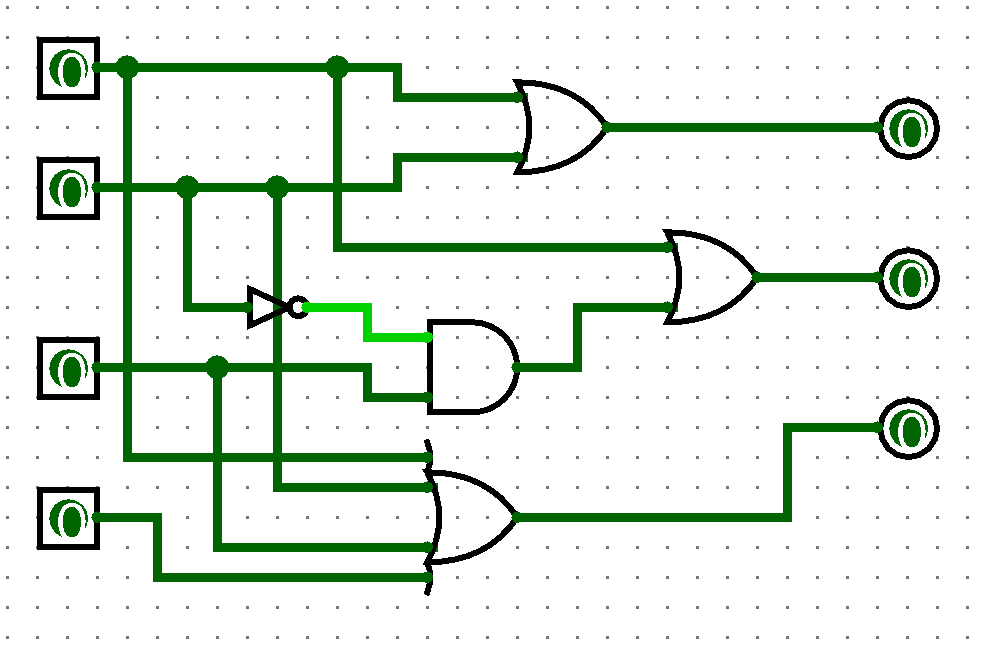
\includegraphics[height = 0.30\textheight]{recursos/Ejercicio4/CircuitoDecodificador.png}\par
    \caption*{Circuito Decodificador}
\end{figure*}

\chapter*{Ejercicio5}
\section*{5. Disenar un circuito secuencial flip-flop SR, pero utilizando circuitos NAND y
verificar que el resultado es el mismo que con puertas NOR.}

\begin{enumerate}
    \item 
Circuito Flip-Flop SR usando compuertas NAND:
\end{enumerate}

\begin{center}
    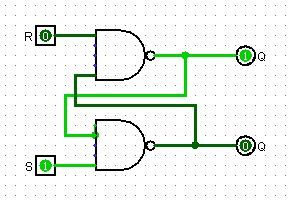
\includegraphics[width=0.5\textwidth]{recursos/Ejercicio5.png}
\end{center}

\begin{enumerate}
    \item 
    Tabla de verdad donde se muestra que es correcto el circuito:
\end{enumerate}


\begin{center}
    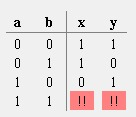
\includegraphics[width=0.5\textwidth]{recursos/TablaEjercicio5.png}
\end{center}
    


\chapter*{Expresar las siguientes oraciones como fórmulas de la lógica de predicados; indicar las constantes, las variables, los cuantificadores y su alcance:}
\chapter*{Ejercicio 7}

\textbf{7.}  Por cada formula: 
\begin{enumerate}
    \item Clasificar la presencia de variables en libres y ligadas
    \item Indicar el alcance del cuantificador
\end{enumerate}
\textcolor{red}{a)} \[ R(x, y) \land L(y) \] \\
\begin{enumerate}
    \item \textbf{Variables Libres:} x, y\\
    \textbf{Variables Ligadas:} No hay variables ligadas (ya que no hay cuantificadores)
    \item No hay cuantificadores
\end{enumerate}

\textcolor{red}{b)} \[ \forall x \, R(x, f(x, y)) \land L(y) \]
\begin{enumerate}
    \item \textbf{Variables Libres:} y \\
    \textbf{Variables Ligadas:} x
    \item EL alcance de $\forall x$ es $R(x, f(x, y))$
\end{enumerate}

\textcolor{red}{c)} \[ \exists x \, \exists y \, R(x, y) \land L(x, y) \]
\begin{enumerate}
    \item \textbf{Variables Libres:} x,y de $L(x, y)$ \\
    \textbf{Variables Ligadas:} x,y de $R(x, y)$
    \item EL alcance de $\exists x$ y de $\exists y$ es $R(x, y)$
\end{enumerate}

\textcolor{red}{d)} \[ \exists y \, L(x, y) \lor \exists z \, R(x, z) \]
\begin{enumerate}
    \item \textbf{Variables Libres:} x\\
    \textbf{Variables Ligadas:} y de $L(x, y)$ y z de $R(x, z)$
    \item EL alcance de  $\exists y$ es $L(x, y)$, y el Alcance de $\exists z$ es $R(x, z)$
\end{enumerate}

\textcolor{red}{e)} \[ \exists y \, R(a, y) \lor L(a) \]
\begin{enumerate}
    \item \textbf{Variables Libres:} a \\
    \textbf{Variables Ligadas:} y de $R(a, y)$
    \item EL alcance de $\exists y$ es $R(a, y)$
\end{enumerate}

\textcolor{red}{f)} \[ D (f(x, y)) \lor \forall z \, R(z, r(y)) \]
\begin{enumerate}
    \item \textbf{Variables Libres:} x,y\\
    \textbf{Variables Ligadas:} z de $R(z, r(y))$
    \item EL alcance de $\forall z$ es $R(z, r(y))$
\end{enumerate}

\textcolor{red}{f)} \[ \forall x \, (L(x) \rightarrow R(a, x) \land C(x, a)) \]
\begin{enumerate}
    \item \textbf{Variables Libres:} a\\
    \textbf{Variables Ligadas:} x
    \item EL alcance de $\forall x$ es $L(x) \rightarrow (R(a, x) \land C(x, a))$
\end{enumerate}

\textcolor{red}{h)} \[ R(x, y, z) \land \exists y \, R(y, x, z) \rightarrow \forall x \, I(x, y) \]
\begin{enumerate}
    \item \textbf{Variables Libres:} x,y,z de $R(x, y, z)$, x,z de $R(y, x, z)$, y de $I(x, y)$ \\
    \textbf{Variables Ligadas:} y de $R(y, x, z)$ y x de $I(x, y)$
    \item EL alcance de $\exists y$ es $R(y, x, z)$ , y de $\forall x$ es $I(x, y)$
\end{enumerate}

\textcolor{red}{i)} \[ \forall x \, (C(x, z) \land R(x, y)) \rightarrow C(y, z) \]
\begin{enumerate}
    \item \textbf{Variables Libres:} z,y de $C(x, z) \land R(x, y)$ y $y$,z de $C(y, z)$\\
    \textbf{Variables Ligadas:x de $C(x, z) \land R(x, y)$} 
    \item EL alcance de $\forall x$ es $C(x, z) \land R(x, y)$
\end{enumerate}

\textcolor{red}{j)} \[ \forall x \, \exists z \, I(x, z) \rightarrow C(z, y) \land D(y) \]
\begin{enumerate}
    \item \textbf{Variables Libres:} z,y de $(C(z, y) \land D(y))$\\
    \textbf{Variables Ligadas:} x de $I(x, z)$
    \item EL alcance de $\forall x$ y de $\exists x$ es $I(x, z)$
\end{enumerate}

\end{document}